\documentclass[10pt, a4paper]{article}
\usepackage{tabulary}
\usepackage[a4paper,includeheadfoot,margin=2cm]{geometry}
\usepackage{graphicx}
\usepackage{float}

\begin{document}
\title{Text-as-Data Assessed Coursework}
\author{Stuart Reilly - 2258082R}
\date{\today}
\maketitle

\section{Part A}
\subsection{Question 1}

The normalization used for title, author and body removes all non-alphanumeric charactes and lowers the case of the letters.
Author is not case-sensitive and does not contain punctuation, as they have to be used in the URLs for user's profile page,
such as https://reddit.com/u/username.
Title and body can both contain punctuation and are case-sensitive, but the punctuation and case do not provide useful
information for the identification of the subreddit.
This is because punctuation and case are used solely to follow English syntax.

\begin{figure}[H]
	\caption{Results using One-Hot encoding vectorizer}
	\begin{center}
		\begin{tabulary}{\textwidth}{|L|L|L|L|L|}
			\hline
			Classifer           & Accuracy  & Precision & Recall    & F1        \\
			\hline
			Most Frequent       & \(0.230\) & \(0.050\) & \(0.012\) & \(0.019\) \\
			Random              & \(0.101\) & \(0.059\) & \(0.054\) & \(0.055\) \\
			Logistic Regression & \(0.690\) & \(0.582\) & \(0.717\) & \(0.619\) \\
			SVC                 & \(0.230\) & \(0.050\) & \(0.012\) & \(0.019\) \\
			BernoulliNB         & \(0.304\) & \(0.085\) & \(0.069\) & \(0.063\) \\
			\hline
		\end{tabulary}
	\end{center}
	\label{fig:one_hot}
\end{figure}

\begin{figure}[H]
	\caption{Confusion Matrix for the Logistic Regression classifier with One-Hot encoding vectorization}
	\begin{center}
		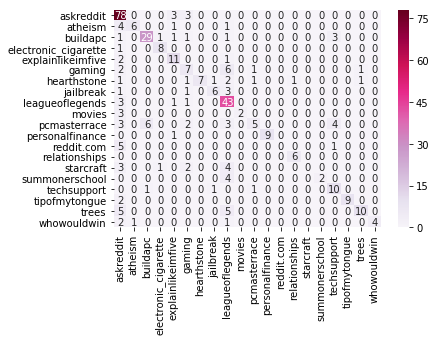
\includegraphics[width=.6\linewidth]{q1_one_hot}
	\end{center}
	\label{fig:one_hot_mat}
\end{figure}

\begin{figure}[H]
	\caption{Results using TF-IDF vectorizer}
	\begin{center}
		\begin{tabulary}{\textwidth}{|L|L|L|L|L|}
			\hline
			Classifer           & Accuracy  & Precision & Recall    & F1        \\
			\hline
			Most Frequent       & \(0.230\) & \(0.050\) & \(0.012\) & \(0.019\) \\
			Random              & \(0.093\) & \(0.037\) & \(0.037\) & \(0.036\) \\
			Logistic Regression & \(0.575\) & \(0.389\) & \(0.658\) & \(0.423\) \\
			SVC                 & \(0.230\) & \(0.050\) & \(0.012\) & \(0.019\) \\
			BernoulliNB         & \(0.304\) & \(0.085\) & \(0.069\) & \(0.063\) \\
			\hline
		\end{tabulary}
	\end{center}
	\label{fig:tfidf}
\end{figure}

\begin{figure}[H]
	\caption{Confusion Matrix for the Logistic Regression classifier with TF-IDF vectorizer}
	\begin{center}
		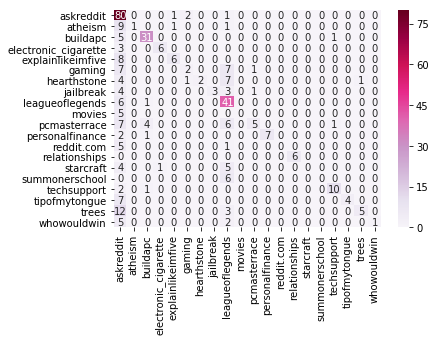
\includegraphics[width=.6\linewidth]{q1_tfidf}
	\end{center}
	\label{fig:tfidf_mat}
\end{figure}

Based on data in Figures \ref{fig:one_hot} and \ref{fig:tfidf}, the best classifier for both vectorizers is Logistic Regression
and the best vectorizer is One-Hot Encoding.
TF-IDF vectorizer is implemented as a CountVectorizer and a TfidfTransformer, therefore is a regularized version of One-Hot encoding.
Regularizing One-Hot encoding removes abnormalities from the data, which changes the result, in this case for the worse.


\begin{figure}[H]
	\caption{Graph of subreddit's F1 Scores using the Logistic Regression classifier with TF-IDF vectorizer}
	\begin{center}
		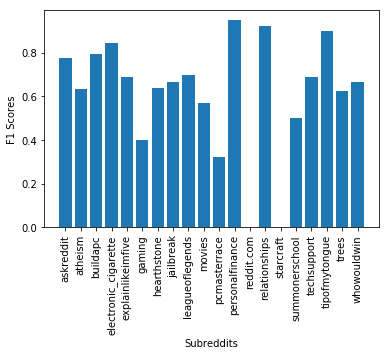
\includegraphics[width=.7\linewidth]{q1_one_graph}
	\end{center}
	\label{fig:f1_graph}
\end{figure}

\subsection{Question 2}
\begin{figure}[H]
	\caption{Confusion Matrix for parameter tuned Logistic Regression classifier with TF-IDF vectorizer}
	\begin{center}
		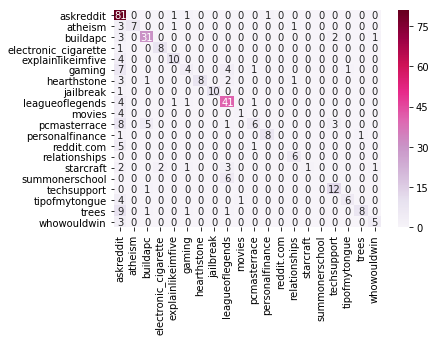
\includegraphics[width=.6\linewidth]{q2_mat}
	\end{center}
	\label{fig:tune_mat}
\end{figure}

Figure \ref{fig:tune_mat} shows the model often incorrectly predicts 'r/askreddit', but the each subreddit is more often
predicted successfully then not.
'r/summonerschool' is never successfully predicted, and is always predicted to be 'r/leagueoflegends'.
This is likely due to how both subreddits are focused around League of Legends, and as such have very similar posts.

\begin{figure}[H]
	\caption{Confusion matrix for parameter tuned Logistic Regression classifier with TF-IDF vectorizer with two extra features}
	\begin{center}
		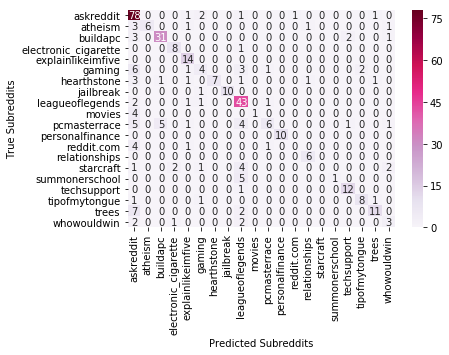
\includegraphics[width=.6\linewidth]{q2_mat_final}
	\end{center}
\end{figure}

The two new features added are the length of each thread and the length of all posts combined.
This reduced the number of incorrectly predicted '/r/askreddit' per subreddit, but increased the spread of incorrectly predicted
'r/askreddit'.

\section{Part B}
\subsection{Question 3}

\begin{figure}[H]
	\caption{Precision, recall and F1-scores of each class using Logistic Regression classifier with TF-IDF vectorizer}
	\begin{center}
		\begin{tabulary}{\textwidth}{|L|L|L|L|}
			\hline
			Class            & Precision & Recall    & F1-score \\
			\hline
			agreement        & \(0.182\) & \(0.542\) & \(0.272\) \\
			announcement     & \(0.008\) & \(0.750\) & \(0.016\) \\
			answer           & \(0.830\) & \(0.509\) & \(0.631\) \\
			appreciation     & \(0.590\) & \(0.764\) & \(0.666\) \\
			disagreement     & \(0.016\) & \(0.270\) & \(0.029\) \\
			elaboration      & \(0.180\) & \(0.301\) & \(0.225\) \\
			humor            & \(0.009\) & \(0.308\) & \(0.017\) \\
			negativereaction & \(0.023\) & \(0.368\) & \(0.043\) \\
			other            & \(0.056\) & \(0.457\) & \(0.100\) \\
			question         & \(0.464\) & \(0.543\) & \(0.500\) \\
			\hline
		\end{tabulary}
	\end{center}
\end{figure}

\begin{figure}[H]
	\caption{Confusion Matrix for discorse prediction}
	\begin{center}
		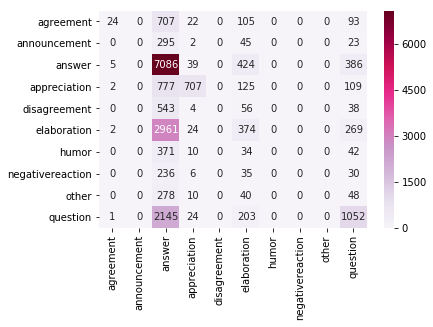
\includegraphics[width=.6\linewidth]{q3_mat}
	\end{center}
\end{figure}

\subsection{Question 4}

\begin{figure}[H]
	\caption{Accuracy, Precision, Recall and F1 scores of additional features}
	\begin{center}
		\begin{tabulary}{\textwidth}{|L|L|L|L|L|}
			\hline
			Feature   & Accuracy & Precision & Recall & F1 Score \\
			\hline
			Metadata  & 0.385    & 0.104     & 0.118  & 0.076 \\
			Content   & 0.556    & 0.241     & 0.422  & 0.248 \\
			Structure & 0.420    & 0.118     & 0.077  & 0.088 \\
			Author    & 0.454    & 0.143     & 0.085  & 0.106 \\
			Thread    & 0.408    & 0.106     & 0.066  & 0.070 \\
			Manual    & 0.507    & 0.237     & 0.465  & 0.253 \\
			\hline
			Combined  & 0.590    & 0.330     & 0.504  & 0.356 \\
			\hline
		\end{tabulary}
	\end{center}
\end{figure}

Subreddit is a metadata feature which adds the subreddit the post is from to the classification.
This aids classification as different subreddits are more likely to have specific types of posts, for example
/r/askreddit is extremely likely to have posts which are questions and answers, whereas /r/dankmemes is likely
to contain humor and negative reaction.
The subreddit feature is implemented using a pipeline containing a custom transformer, ItemSelector, which extracts the subreddit 
from the post objects and a TF-IDF vectorizer to normalize and vectorize the subreddit.

Word ngrams is a content feature which analyses the words and the combination of words used in posts.
Since some classes of posts contain specific words, such as 'what' for questions and 'yes' for answers, word ngrams will aid the classification.
Combinations of words such as 'Not exactly' are likely to be in elaboration posts and 'Thank you mate' in appreciation posts.
The feature is implemented using a pipeline containing an ItemSelector, which extracts the post body, and a TF-IDF vectorizer, 
initialised with the ngram\_range argument given as (1,3), to normalize and vectorize the post body.

Post depth is a structure feature which analyses the depth in a thread a post is.
A post with a depth of 0 is extremely unlikely to be an answer post and a post with a non-zero post depth is unlikely to be an announcement.
This feature is implemented using a pipeline containing an ItemSelector, which extract the 'post\_depth' from the post object, and a
FunctionTransformer, which runs a function which reshapes the data into a column vector.

Is current author the author of the initial post is an author feature which analyses if the initial post's author continues
in the comments of the post.
A post with the same author as the initial post is likely to be a positive/negative reaction or a question.
This feature is implemented by adding a new column to the DataFrame containing the posts, which contains a boolean representing
if the current post's author is the same as the initial post.
Before the loop which adds the posts to the DataFrame, the posts are first iterated over until a post with a post depth of 0 or
no post depth given, storing the author of this post as the post found is the initial post.
During the loop which adds the posts to the DataFrame, the new column is added with true if the current post's author is the same
as the stored initial author, or false otherwise.
A pipeline is added to the main pipeline which contains an ItemSelector, which extracts this new column, and a FunctionTransformer,
which runs a function which reshapes the data into a column vector.

Self-post or Link-post is a thread feature which takes into account if the thread starts with a link to another web page or a text post.
A post which is a Link-post is unlikely to be an elaboration or agreement post.
This feature is implemented by adding a new column to the DataFrame containing the posts, which contains a boolean representing
if the post is a self post.
The value for this new column is the value from the 'is\_self\_post' entry in the thread object the post is extracted from.
A pipeline is added to the main pipeline which contains an ItemSelector, which extracts this new column, and two FunctionTransformers.
The first FunctionTransformer reshapes the data into a column vector and the second replaces all NaN values with false.

The combined feature of subreddit and post body is a manually defined feature which links the subreddit and the post body into a
single feature.
A post on gaming subreddit will contain vocabulary, which is unique to the game the subreddit is based on, which might have different
meaning is different subreddits.
For example, the phrase 'zerg rushing' can be used to mean something is swarming something, or it can mean someone is using a 
disrespectful tactic to get an edge.
These two different means can change the class of a post, depending on which is used.
This feature is implemented using a FeatureUnion of two pipelines.
One pipeline uses an ItemSelector to extract the subreddit and a TF-IDF vectorizer to normalize and vectorize the subreddit.
The other pipeline uses an ItemSelector to extract the post body and a TF-IDF vectorizer to normalize and vectorize the post body.

\begin{figure}[H]
	\caption{Chart showing the feature weights of each class of post}
	\begin{center}
		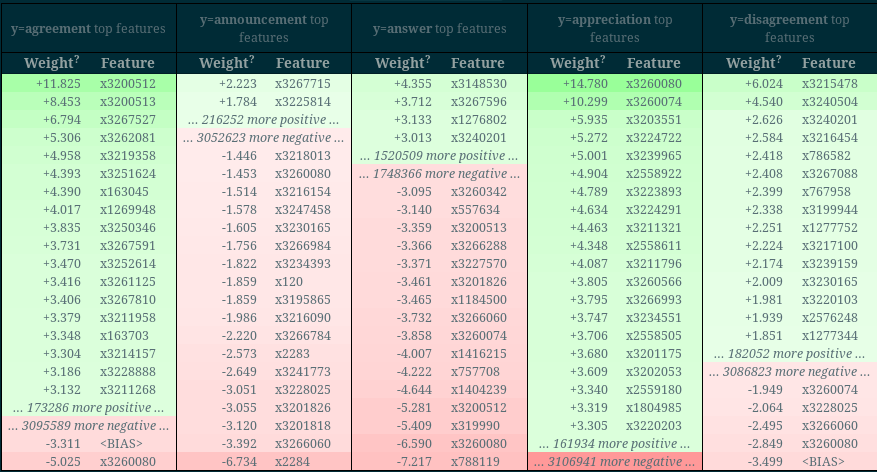
\includegraphics[width=.8\linewidth]{q4_tab_1}
		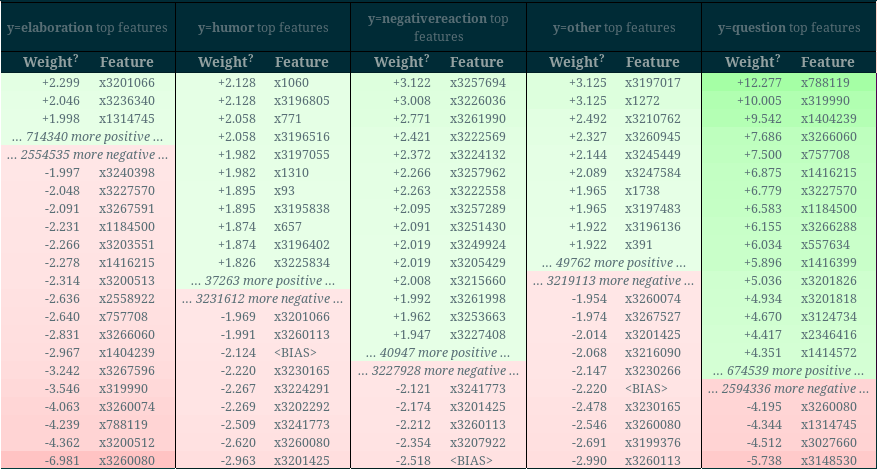
\includegraphics[width=.8\linewidth]{q4_tab_2}
	\end{center}
\end{figure}

\end{document}

%Evaluation for: Pipeline
%Classifier 'Pipeline' has Acc=0.590 P=0.330 R=0.505 F1=0.356
%Best Confusion Matrix
%                  precision    recall  f1-score   support
%
%       agreement      0.216     0.553     0.310       371
%    announcement      0.460     0.691     0.553       243
%          answer      0.849     0.603     0.705     11184
%    appreciation      0.625     0.772     0.691      1392
%    disagreement      0.037     0.369     0.068        65
%     elaboration      0.318     0.405     0.356      2854
%           humor      0.035     0.271     0.062        59
%negativereaction      0.046     0.311     0.080        45
%           other      0.048     0.439     0.086        41
%        question      0.664     0.639     0.651      3558
%
%       micro avg      0.590     0.590     0.590     19812
%       macro avg      0.330     0.505     0.356     19812
%    weighted avg      0.698     0.590     0.628     19812
